%BAB-1 Laporan KP

\chapter{PENDAHULUAN}

\section{Latar Belakang Masalah}

Perkembangan teknologi serta ilmu pengetahuan pada masa ke masa semakin berkembang. Perkembangan ini berjalan seiring dengan penelitian-penelitian di berbagai disiplin ilmu khususnya dalam bidang instrumentasi dan kendali. Hal ini dapat dilihat dari banyaknya penggunaan sistem instrumentasi dan kendali dalam dunia industri seperti pengguanaan robot dalam menyelesaikan pekerjaan manusia. Untuk itu perancangan robot merupakan salah satu solusi untuk memenuhi tuntutan dalam membantu kebutuhan manusia \cite{Faris2012}.

Pemilihan robot untuk menggantikan pekerjaan manusia tidak terlepas dengan berbagai kelebihannya. Salah satu kelebihannya, sebuah robot dapat melakukan suatu pekerjaan yang sama dan berulang tanpa merasakan lelah seperti halnya manusia. Pekerjaan ini lah yang biasa ditemukan dalam bidang industri khususnya pada bagian produksi. Robot dengan sistem lengan robot (\emph {robot arm system}) merupakan salah satu jenis robot yang dominan berada dalam bidang industri\cite{Bimantaka2014}. 

Robot lengan memiliki berbagai jenis salah satunya adalah robot \emph{selective compilance assembly robot arm} (SCARA Serpent). Dalam melakukan pergerakan, robot SCARA Serpent umumnya bergerak menuju sebuah koordinat posisi ($x, y$) yang dibantu dengan sebuah persamaan kinematika. Persamaan kinematika yang diguanakan adalah \textit{inverse kinematic} dengan masukan berupa titik koordinat kartesian \textit{($x$,$y$)} dan keluaran berupa nilai sudut untuk mengendalikan motor DC pada \textit{shoulder} dan \textit{elbow}.

Pada laporan penelitian KP, penelitian lebih difokuskan terhadap gerak kinematika dari robot serta perancangan antarmuka untuk memudahkan dalam mengoperasikan robot. Robot SCARA Serpent telah banyak dijadikan sebagai objek penelitian, salah satu penelitian robot SCARA Serpent Serpent yang populer merupakan penelitian tentang menjadikan robot SCARA Serpent menjadi robot yang dapat memindahkan objek tergantung warna dari masing-masing objek. Dengan penelitian tersebut maka robot SCARA Serpent dapat memiliki fungsi lebih banyak serta dapat ditempatkan ke dalam dunia industri.

Dalam berbagai penelitian tentang robot SCARA Serpent, banyak ditemukan beberapa masalah yang sering terjadi terkait robot SCARA Serpent. Masalah yang umum terjadi adalah terbatasnya pergerakan pada garis vertikal. Robot SCARA Serpent dalam melakukan pergerakan vertikal dijalankan menggunakan \textit{joint prismatic} yang terletak pada \textit{end effector}. Dengan begitu pergerakan vertikal dalam robot dibatasi oleh minimnya panjang \textit{link} pada \textit{end-effector} yang menyebabkan objek yang dapat diambil oleh robot SCARA Serpent tidak dapat terlalu tinggi.

Dalam mengendalikan sebuah robot dibutuhkan \textit{platfrom} antarmuka sebagai jembatan antara \textit{user} dengan \emph{hardware}. Dalam penelitian ini program antarmuka dirancang menggunakan \textit{software} Processing IDE. Penggunaan Processing IDE sebagai antarmuka karena memiliki beberapa keunggulan, seperti mudahnya sarana komunikasi terhadap \emph {hardware} yang digunakan. Oleh karena itu, pada program kerja praktik ini dilakukan analisis kinematika robot SCARA Serpent dengan perancangan antarmuka berbasis  Processing IDE.\\


\section{Tujuan Penelitian}
Adapun tujuan dalam melaksanakan penelitian "Kinematika dan Antarmuka Robot SCARA Serpent" adalah sebagai berikut:

\subsection{Secara Umum}
\begin{enumerate}
	\item Merancang\emph{ arm manipulator robot} SCARA Serpent berbasis Arduino Mega 2560.
	\item Memahami dan mengimplementasikan antarmuka Processing \textit{integrated development environment} (IDE).
	\item Mengimplementasikan kinematika pada \emph{arm manipulator robot} SCARA Serpent.
\end{enumerate}
\subsection{Tujuan Khusus}
Untuk memenuhi salah satu syarat kelulusan dalam menempuh pendidikan Program   Diploma III Teknologi Listrik, Sekolah Vokasi, Universitas Gadjah Mada. 


\section{Batasan Penelitian}
Pembatasan masalah diperlukan untuk mempermudah pelaksanaan penulisan laporan kerja praktik (KP) sehingga tidak menyimpang dari judul laporan. Lingkup pembatasan masalah dalam laporan KP ini dibatasi pada:

\begin{enumerate}
	
	\item Akurasi dari robot lengan dipengaruhi oleh spesifikasi dan torsi dari masing-masing motor DC pada \emph{ joint.}
	\item  Rancangan mekanik yang sudah tersusun dari awal sehingga tidak dapat diubah lagi. 
	\item Besar objek yang dapat dibawa oleh \textit{gripper} memiliki ukuran yang terbatas.
	\item Komunikasi antara Processing IDE dan \textit{hardware} menggunakan komunikasi serial yang dihubungkan dengan kabel USB.
	
\end{enumerate}

\section{Metode Kerja Praktik}
Metodologi adalah suatu cara yang digunakan untuk memperoleh data yang akurat, baik melalui observasi lapangan maupun dari \emph {datasheet} setiap alat yang digunakan. Observasi juga dilakukan dengan meninjau jurnal-jurnal dan konsultasi mengenai penelitian yang dilakukan. Pada bagian ini dijelaskan meliputi waktu dan tempat penelitian, alat dan bahan penelitian, rancangan alat, metode penelitian dan prosedur penelitian. Penjelasan lebih rinci tentang metodologi penelitian akan dijelaskan sebagai berikut: 

\begin{enumerate}
	\item Waktu dan Tempat Penelitian \\
	Penelitian dilakukan di Labolatorium Instrumentasi dan Kendali Departemen Teknik Elektro dan Informatika (DTEDI) Sekolah Vokasi Universitas Gadjah Mada pada bulan Juli sampai bulan Agustus 2019.
	
	\item Alat dan Bahan \\
	Peralatan yang digunakan dalam KP adalah personal \textit{computer} (PC), Arduino Mega 2560, transformator AC 5A, \textit{converter} AC to DC, modul DC to DC \textit{converter} LM2596, IC TIP 31, multimeter,\textit{ valve pneumatic}, \textit{driver} motor EMS 30A dan catu daya AC 220 Volt. Sedangkan bahan yang digunakan adalah motor DC yang terpasang di setiap \emph {joint} robot lengan serta \textit{valve relay pneumatic} untuk mengkontrol tekananan udara.
	
	\item  Pengumpulan Data \\
	Studi pustaka dilakukan dengan cara mengumpulkan buku-buku, dokumen, serta jurnal-jurnal berbentuk \emph{e-book} yang berkaitan dengan robot lengan. Selain itu \emph{datasheet} dari setiap komponen juga ditinjau. Data-data tersebut menjadi referensi untuk merancang, membuat, dan menguji alat. 
	
	Konsultasi dilakukan untuk mengumpulkan data melalui tanya jawab atau berdiskusi dengan pihak yang mengetahui dan menguasai segala permasalahan yang dihadapi dalam merancang, membuat, dan menguji robot lengan SCARA Serpent. Dalam metode ini penulis berdiskusi dengan dosen pembimbing KP. 
	
	\item Metode Penelitian \\
	Metode penelitian yang dilakukan meliputi; pengujian tegangan DC to DC \textit{converter}, pengujian motor DC, pengujian \textit{driver} motor DC EMS 30A, pengujian rangkaian \textit{switching valve pneumatic}, pengujian kinematika balik, pengujian dengan kendali proposional serta pengambilan data dan analisa data.
	
	\item Prosedur Penelitian\\
	Prosedur penelitian adalah langkah-langkah dalam menyelesaikan KP yang akan disajikan dalam bentuk diagram alir pada Gambar \ref{pic.diagramalir}.
	
	\begin{figure}[H]
		\centering
		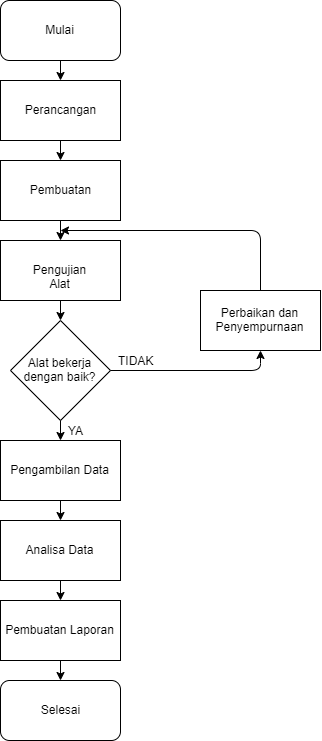
\includegraphics[width=7cm]{gambar/flowchart.png}
		\caption{ Diagram Alir Prosedur Penelitian}
		\label{pic.diagramalir}
	\end{figure}
	
	
\end{enumerate}

\section{Sistematika Penulisan}
Penulisan laporan KP ini dilakukan dengan mengikuti sistematika sebagai berikut:\\
\noindent
\textbf{BAB I\hspace*{0.6cm} PENDAHULUAN}\\
\noindent
Merupakan pendahuluan dari laporan KP yang menjelaskan latar belakang, tujuan, batasan masalah dan metodologi penyusunan laporan KP.\\
\noindent
\textbf{BAB II\hspace*{0.5cm} LANDASAN TEORI}\\
\noindent
Memuat gambaran umum robot lengan, \emph {degress of freedom}, konfigurasi robot lengan, \emph{wrist} dan \textit{end-effector}, kinematika, pengertian dan prinsip kerja Processing IDE sebagai antarmuka robot lengan, dan prinsip kerja setiap piranti yang digunakan dalam pembuatan robot lengan. \\
\textbf{BAB III\hspace*{0.375cm}  PERANCANGAN SISTEM}\\
\noindent
Memuat perancangan sistem secara umum, perancangan perangkat keras berupa elektronis dari robot lengan, perancangan perangkat lunak berupa pengolahan \textit{graphical user interface} (GUI) menggunakan Processing IDE, sistem kinematika balik untuk robot lengan, dan integrasi keseluruhan program. \\
\textbf{BAB IV\hspace*{0.4cm}  PENGUJIAN DAN ANALISA KERJA SISTEM }\\
\noindent
Memuat pengujian tegangan DC to DC \textit{converter}, pengujian motor DC, pengujian \textit{driver} motor DC EMS 30A, pengujian rangkaian \textit{switching valve pneumatic}, pengujian kinematika balik, pengujian dengan kendali proposional, serta pengambilan data dan analisa data hingga pada pengujian menyeluruh.\\
\textbf{BAB V\hspace*{0.6cm} PENUTUP}\\
Memuat tentang kesimpulan dari perancangan, pengujian dan analisis dari sistem kerja robot, serta berisi saran – saran untuk mengembangkan penelitian \emph{ arm manipulator robot} SCARA Serpent lebih lanjut. \\